\chapter{Protocol \\
  \small{\textit{-- Evan Ciok, Sophia DiCuffa, Carson McManus}}
  \index{Chapter!protocol}
  \index{protocol}
  \label{Chapter::Protocol}}

\section{Messaging Protocol}

The Balancer must maintain a maximum of one websocket \index{websocket} connection to each Monolith \index{monolith} node. This implies that the Balancer \index{balancer} must be able to convey the user identity of messages sent to the Monolith.

The client communicates over the websocket with messages in JSON \index{JSON} format \index{format}, so the Balancer should do the same. The Balancer will send messages to the Monolith in the following format:

\begin{verbatim}
	{
		"token": string // the client's auth token
		"room": string // the room the client is in
		"id": string // a unique identifier for the connection
		"message": <JSON object> // literal JSON object received from the client
	}
\end{verbatim}

This will allow the server to relay the message without having to do a serialization round trip. The Monolith can send messages to individual clients by sending the message to the Balancer in the following format:

\begin{verbatim}
	{
		"room": string // the room the client is in
		"id": string // a unique identifier for the connection
		"message": <JSON object> // the literal JSON object to send to the client.
	}
\end{verbatim}

For broadcast messages, the Monolith can omit the ``id'' field.

\begin{verbatim}
	{
		"room": string // the room to broadcast to
		"message": <JSON object> // literal JSON object to send to all clients
	}
\end{verbatim}



\subsection{Messages sent during Join and Leave}

When a client opens a websocket connection, the client must immediately send an "auth" message. This is because the browser's websocket API does not allow for the client to send headers with the initial connection request.

\begin{verbatim}
	{
		"action": "auth",
		"token": string // the client's auth token
	}
\end{verbatim}

Once the the Balancer, receives this message, it must send a message to the Monolith to update the room's state.

\begin{verbatim}
	{
		"token": string // the client's auth token
		"room": string // the room the client is joining
		"message": {
			"action": "req",
			"request": {
				type: RoomRequestType.JoinRequest;
			}
		}
	}
\end{verbatim}

\begin{figure}[h!]
	\centering
	\scalebox{0.57}{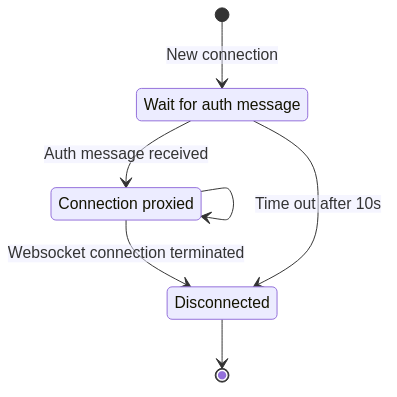
\includegraphics{Figures/client-connection-state.png}}
	\caption{State diagram for Websocket connections from clients to the Balancer.}
	\label{fig:client-connection-state}
\end{figure}

Similarly, when a client disconnects, the Balancer must send a message to the Monolith to update the room's state.

\begin{verbatim}
	{
		"token": string // the client's auth token
		"room": string // the room the client is leaving
		"message": {
			"action": "req",
			"request": {
				type: RoomRequestType.LeaveRequest;
			}
		}
	}
\end{verbatim}

These messages conform to the the protocol defined by the types in the \href{https://github.com/dyc3/opentogethertube/blob/master/common/models/messages.ts}{OTT monolith here}.

\section{Messages sent during Monolith connection startup}

When a Monolith starts up, and it has balancers configured, it must initiate a websocket connection to each of the balancers. The Monolith must send an "init" message to the Balancer to inform it of the port that it is listening for HTTP requests on, and an auth token to verify authenticity.

Once the Balancer receives this message, the connection is considered established, and the Monolith and Balancer can begin sending messages to each other.